% \documentclass{standalone}

% \input{../tikz_header}

% \begin{document}


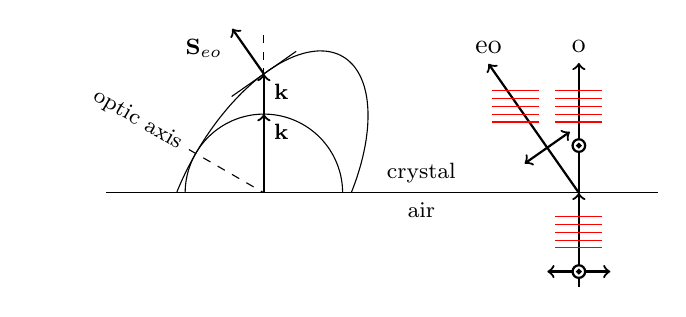
\begin{tikzpicture}
    %\useasboundingbox (-2.5,-1.5) rectangle (3,2.3);
    %\draw (-2.5,-1.5) rectangle (3,2.3);
 
    \pgfmathsetmacro{\mya}{1}
    \pgfmathsetmacro{\myb}{2}
    \pgfmathsetmacro{\theta}{35}

    \begin{scope}
        \clip(-3,0) rectangle (2,2);
        \begin{scope}[rotate=-30]
            \draw[] plot[variable=\x,domain=0:360,smooth,samples=51] ({\mya*cos(\x)}, {\myb* sin(\x) });
            \draw[] plot[variable=\x,domain=0:360,smooth,samples=51] ({\mya*cos(\x)}, {\mya* sin(\x) });
            \draw[dashed] (-1.1,0) node[rotate=-30, anchor=east] {\footnotesize optic axis}  --  (+1.5,0) ;
        \end{scope}    
    \end{scope}    

    \draw(-2,0) -- (2,0);
    \node [above] at (2,0) {\footnotesize crystal};
    \node [below] at (2,0) {\footnotesize air};

    \draw[->, thick] (0,0) -- (0,1) node[anchor=north west] {\footnotesize $\mathbf{k}$};
    \draw[->, thick] (0,0) -- (0,1.51) node[anchor=north west] {\footnotesize $\mathbf{k}$};
    \draw[dashed] (0,0) -- (0,2) ;
    \draw[thin] (0,1.51) -- ++(\theta:0.5);
    \draw[thin] (0,1.51) -- ++({\theta-180}:0.5);
    \draw[->, thick] (0,1.51) -- ++({\theta+90}:0.7) node[anchor=north east] {\footnotesize$\mathbf{S}_{eo}$};

    \begin{scope}[xshift=40mm]
        \draw(-2,0) -- (1,0);
        \draw[->, thick ] (0,0) -- ++({\theta+90}:2) node[anchor=south] {eo} ;
        \draw[-> , thick] (0,0) -- ++(90:1.65) node[anchor=south] {o} ;
        \draw[<-, thick ] (0,0) -- ++(-90:1.2) ;

        \draw[<->, thick] (-0.4, -1) -- (0.4, -1);
        \draw[fill=white, thick] (0,-1) circle (0.08);
        \draw[fill=black, thick] (0,-1) circle (0.02);

        \draw[fill=white, thick] (0,0.6) circle (0.08);
        \draw[fill=black, thick] (0,0.6) circle (0.02);

        \draw[->, thick] (\theta+90:0.7) --++ (\theta: 0.35);
        \draw[->, thick] (\theta+90:0.7) --++ (\theta+180 :0.35);

        \pgfplotsinvokeforeach{0.3,0.4,...,0.7}{
            \draw [red] (-0.3,-#1) -- (0.3,-#1);
            \draw [red] (-0.3,{0.6+#1}) -- (0.3,{0.6+#1});
            \draw [red] (-1.1,{0.6+#1}) -- (-0.5,{0.6+#1});
        }

    \end{scope}
        


\end{tikzpicture}


%\end{document}